\documentclass[a4paper,10pt]{scrreprt}

% Basics
\usepackage{graphicx}
\usepackage[T1]{fontenc}
\usepackage[ngerman]{babel}
\usepackage{url}
\usepackage{amssymb}
\usepackage{color}
\usepackage{ifthen}

% clickable and fillable PDF
\usepackage{hyperref}
\hypersetup{%
  bookmarksnumbered,
  bookmarksopen=true,
  bookmarksopenlevel=0,
  breaklinks=true,
  colorlinks=true,
  allcolors=black,
  hypertexnames=true,
  linktocpage=true,
  pageanchor=true,
  pdfhighlight=/O,
  pdfpagemode=UseOutlines,
  pdfstartview=FitV,
  plainpages=false
}

% keine Ahnung
\usepackage[parfill]{parskip}

% larger pages
\usepackage[cm]{fullpage}

% numbered lines
\usepackage{lineno}
\renewcommand\linenumberfont{\normalfont\tiny}

% allows to define compact lists
\usepackage{paralist}
\newenvironment{niceitemize}
{
\begin{list}{\labelitemi}{\leftmargin=0em}}
{\end{list}}
\renewcommand{\labelitemi}{--}
\newcounter{nicecount}
\newenvironment{niceenumerate}
{
\begin{list}{\arabic{nicecount}.}{\usecounter{nicecount}\leftmargin=0em\itemsep=0em\topsep=0.5em}}
{\end{list}}

% framed environment
\usepackage{framed}
\definecolor{shadecolor}{gray}{0.95}
\definecolor{porange}{cmyk}{0,0.5,1.0,0}
\definecolor{pgray}{RGB}{88,88,90}

% to display current time
\usepackage{uhrzeit}

% layout hacks
\usepackage{microtype}
\clubpenalty = 10000
\widowpenalty = 10000
\displaywidowpenalty = 10000

% control title fonts
\usepackage[compact]{titlesec}
\titleformat*{\subsection}{\large\bfseries\sffamily\color{pgray}}
\titleformat*{\subsubsection}{\bfseries\sffamily\color{pgray}}
\titlespacing{\section}{0pt}{0pt}{*0}
\titlespacing{\subsection}{0pt}{10pt}{*0}

% reduce chapter margin
\renewcommand*\chapterheadstartvskip{\vspace*{-3\topskip}} 

% control TOC entries
\usepackage[titles]{tocloft}
\setlength{\cftbeforechapskip}{0.25em}

% no numbering of chapters, sections, etc.
\setcounter{secnumdepth}{-1}

% only show parts and chapters in TOC
\setcounter{tocdepth}{0}

% choose default fonts
\usepackage{fontspec,xltxtra,xunicode}
\defaultfontfeatures{Mapping=tex-text}

\setromanfont[Mapping=tex-text]{DejaRip}
\setmonofont[Mapping=tex-text]{Menlo}
\setsansfont[Scale=MatchLowercase,Mapping=tex-text]{Conduit ITC Pro}

\renewcommand{\textbf}[1]{\setromanfont[Mapping=tex-text]{DejaRip Bold}{\bfseries #1}\setromanfont[Mapping=tex-text]{DejaRip}}

% enlarge footnotes
\renewcommand{\footnotesize}{\scriptsize}

% indices
\usepackage[makeindex]{splitidx}
\newindex[Anträge nach Nummer]{innummer}
\newindex[Anträge nach Titel]{inantraege}
\newindex[Anträge nach Typ]{intyp}
\newindex[Beantragte Satzungsänderungen]{insatzung}
\usepackage[columns=1,font=small]{idxlayout} 

% background image
\usepackage{wallpaper}

% remove left margin of quotes
\renewenvironment{quote}{\list{}{\leftmargin=2em\rightmargin=0in}\item[]}{\endlist}


%%%%%%%%%%%%%%%%%%%%%%%%%%%%%%%%%%%%%%%%%%%%%%%%%%%%%%%%%%%%%%

\newcommand{\LPTtitel}{}
\newcommand{\LPTantragsteller}{}
\newcommand{\LPTlqfbinitiative}{}
\newcommand{\LPTlqfbvote}{}
\newcommand{\LPTlqfbsummary}{}
\newcommand{\LPTlqfbarea}{}
\newcommand{\LPTrelations}{}
\newboolean{LPTlqfb}
\newboolean{LPTrelated}

\newcommand{\LPTantrag}[1]
{
\input{antraege/#1-meta.tex}

\setcounter{chapter}{#1}

%\chapter*{\vspace{-2.5em}{\LARGE\normalfont Antrag #1}\\\LPTtitel{}%\phantomsection\label{chap:#1}
%}
%\addcontentsline{toc}{chapter}{$\Box$ {\normalfont  #1:} \hyperref[chap:#1]{\LPTtitel{}}}

\chapter[{\normalsize $\Box$ {\normalfont  #1:} \LPTtitel{}}]{{\LARGE\normalfont Antrag #1}\\\vspace{-0.1em}{\LARGE\LPTtitel{}}}\label{chap:#1}

\begin{shaded}
%\vspace{-1em}
Antragsteller: \LPTantragsteller{} \hfill
{\small\url{http://lmv.piraten-mv.de/antrag/#1}}\\
\vspace{-1em}

%\sindex[inantraege]{\LPTtitel{}}
%\sindex[innummer]{#1}
%\sindex[intyp]{\LPTprogrammtyp{}!\LPTtitel{}}
\sindex[inantraege]{\LPTtitel{}@$\Box$ \LPTtitel{} (Antrag #1)}
\sindex[innummer]{#1@$\Box$ Antrag #1: \LPTtitel{}}
\sindex[intyp]{\LPTprogrammtyp{}!$\Box$ \LPTtitel{} (Antrag #1)}

\ifthenelse{\boolean{LPTrelated}}{Beziehung zu anderen Anträgen: \LPTrelations}{}

\ifthenelse{\boolean{LPTlqfb}}{\LPTlqfbarea{}\hfill {\small\url{http://mv.pplf.de/i\LPTlqfbinitiative}}\\\LPTlqfbsummary{}\hfill \LPTlqfbvote{}\\
}{\vspace{0.75em}}

\vspace{-1.75em}
\begin{Form}
\ChoiceMenu[radio,name=#1user]{}{\phantom{.}=zu} Ja
\ChoiceMenu[radio,name=#1user]{}{\phantom{.}=en} Enthaltung
\ChoiceMenu[radio,name=#1user]{}{\phantom{.}=ab} Nein
%\hspace{2em}
\hfill
\ChoiceMenu[radio,name=#1vote]{}{\phantom{.}=an} Angenommen
\ChoiceMenu[radio,name=#1vote]{}{\phantom{.}=zu} Zurückgezogen
\ChoiceMenu[radio,name=#1vote]{}{\phantom{.}=ab} Abgelehnt
\end{Form}\\
\vspace{-0.75em}
\end{shaded}

%\index{inantraege}{\LPTtitel{}@\LPTtitel{} (Antrag #1)}
%\index{innummer}{#1@Antrag #1 (\LPTtitel{})}

\bigskip

%\begin{Form}
%\TextField[name=notes#1,width=\textwidth,height=8em,multiline]{ }
%\end{Form}

%\begin{minipage}{10cm}
\linenumbers

%\addtolength\textwidth{-3\baselineskip}

%\begin{antragstext}

%\begin{adjustwidth}{0cm}{4cm}\leavevmode%
\input{antraege/#1.tex}
%\end{adjustwidth}


%\end{antragstext}

%\end{minipage}

%\par
%\begingroup
%\rightskip12em
%\input{antraege/#1.tex}
%\par
%\endgroup

%\theendnotes

\setcounter{footnote}{0}

\nolinenumbers
\resetlinenumber
\setcounter{section}{0}
}

%%%%%%%%%%%%%%%%%%%%%%%%%%%%%%%%%%%%%%%%%%%%%%%%%%%%%%%%%%%%%%
%%%%%%%%%%%%%%%%%%%%%%%%%%%%%%%%%%%%%%%%%%%%%%%%%%%%%%%%%%%%%%
%%%%%%%%%%%%%%%%%%%%%%%%%%%%%%%%%%%%%%%%%%%%%%%%%%%%%%%%%%%%%%

\newcommand{\LPTupdate}{7. Juli 2012, 15:44 Uhr}

\title{
\includegraphics[scale=1]{icons/logofront}\vspace{2em}\\Antragsbuch für die\\ Landesmitgliederversammlung 2012.2}
%\publishers{}
\subtitle{3.\ November 2012, Kulturhaus, Groß Laasch}
\date{Stand: \today, \uhri{}}

\dedication{\footnotesize Dieses Antragsbuch enthält die an die Antragskommission gestellten Anträge zur Landesmitgliederversammlung ({\footnotesize\url{http://lmv.piraten-mv.de/antraege}}), zuletzt abgerufen am \LPTupdate{}.\bigskip

Antragskommission und Umsetzung: Niels Lohmann\\
Logo: Jesthan Endh\\
Piktogramme: Daniel Bruce (www.entypo.com) bzw.\ Twitter, Inc.\bigskip

{\fontspec[Scale=5]{Entypo} \char"1F545\char"1F546\char"1F54A}\\Piratenpartei Deutschland, Landesverband Mecklenburg-Vorpommern
}

\begin{document}
\maketitle

\begin{abstract}
\null
\vfill

%\begin{minipage}{10cm}
\section*{Hallo liebe Piraten,}%\medskip

die Schlagzahl der Mitgliederversammlungen hat sich zum Ende des Jahren deutlich erhöht. Westmecklenburg, Vorpommern-Greifswald und nun die Landesmitgliederversammlung, gefolgt von Rostock, abermals Westmecklenburg und als Jahresabschluss der Bundesparteitag. Diese sind das Ergebnis der kontinuierlichen strukturellen Arbeit, die wir Piraten im vergangenen Jahr geleistet haben und zeigt auf, wir stark wir uns im letzten Jahr entwickelt haben. Die Mitgliederzahlen haben sich verdoppelt, neue Kreisverbände sind in Gründung und die Aussichten in den Bundestag einzuziehen sind derzeit nicht schlecht. Genügend Motivation ist auch vorhanden, man sehe sich die Vielzahl an Bewerbern für den Vorstand an. Noch viel mehr zeigt es aber, wie ernst wir unsere Mitgliederdemokratie nehmen. Als eines unserer wichtigsten Prinzipien grenzt sie uns methodisch stark von anderen Parteien ab und ist ein Alleinstellungsmerkmal, auf das ich im Hinblick auf die Ständige Mitgliederversammlung in unserem Landesverband besonders stolz bin. Die inhaltliche und strukturelle Entwicklung wird nicht über den Vorstand vorgegeben, sondern wir Mitglieder entscheiden selbst, wie wir unsere Partei weiterentwickeln. Die Ständige Mitgliederversammlung wird heute nach den Wahlen den – hoffentlich – letzten Feinschliff bekommen, um schnellstmöglich auch abseits realer Versammlungen über inhaltliche, politische Standpunkte entscheiden zu können und uns damit politisch noch handlungsfähiger machen.\medskip

Ich wünsche uns eine schöne und erfolgreiche Mitgliederversammlung!\bigskip

  Michael Rudolph
%\end{minipage}

\vfill
\vfill

\begin{tabular}{lll}
{\fontspec[Scale=3]{Entypo} \char"1F4F6} & \textbf{WLAN} & \\
& Name: & \verb|#lmvmv122| \\
& Passwort: & \verb|piratenpartei|\\
& & \\
{\fontspec[Scale=3]{Entypo} \char"1F4C4} & \textbf{Tagesordnung} & \\
& Entwurf: & \url{http://lmv.piraten-mv.de} \\
& Protokoll: & \url{http://lmv.piraten-mv.de/protokoll} \\
& Openslides: & \url{http://openslides.piraten-mv.de} \\
& & \\
{\fontspec[Scale=3]{Entypo Social} \char"F309} & \textbf{Twitter} & \\
& Account: & \verb|@Piraten_MV| \\
& Hashtag: & \verb|#lmvmv122| \\
\end{tabular}


\vfill
\null

%
%als die Vorbereitungen für den Landesparteitag begannen, stellte Niels die Frage in den Raum, ob wir ein Antragsbuch brauchen werden. Ich zweifelte, ob ein solches wirklich nötig sei, da es zu diesem Zeitpunkt nur eine überschaubare Menge an Anträgen gab. Das änderte sich derart, dass hier heute schon fast 50 unterschiedlichste Anträge zu finden sind und ich mich auf einen spannenden Landesparteitag mit inhaltlichen Diskussionen freue.
%
%Alle Anträge auf diesem Parteitag sind das Ergebnis von Engagement, der Investition von Zeit zum Lesen und Reagieren im Liquid Feedback, auf der Mailingliste oder anderen unserer Medien. Sie bilden die Kernaufgaben von uns Piraten: die politische Arbeit. An dieser müssen wir uns messen lassen. Nicht daran, wie viele Infotische wir machen, wie viele Flyer wir verteilen oder wie viele Menschen an unseren Bundesparteitagen teilnehmen. Allein die Inhalte sind es, die eine Partei ausmachen. Wir treten bei einer Wahl an, um mit unseren Inhalten eine Alternative anzubieten und um was zu verändern. Genau hier haben wir den richtigen Weg eingeschlagen, haben jedoch noch viel Potential, was wir nutzen können.
%
%Aber egal ob die Anträge zu Gesundheit, Rettungswesen, Bildung oder zur Satzung; jedem Antrag gingen mitunter viel Überzeugungsarbeit, Recherche und detailverliebten Verbesserungen voraus. Deswegen danke ich an dieser Stelle allen Menschen, die bei den Anträgen direkt oder indirekt mitgewirkt haben. Ich bin mir sicher, dass ich mit ständig steigenden Anzahl an Mitgliedern und auch der bevorstehenden Bundestagswahl 2013 vor keinem Parteitag mehr Bedenken ob fehlender Anträge haben muss.
%
%Eurer\\
%\quad Michael Rudolph
%
%\vfill
%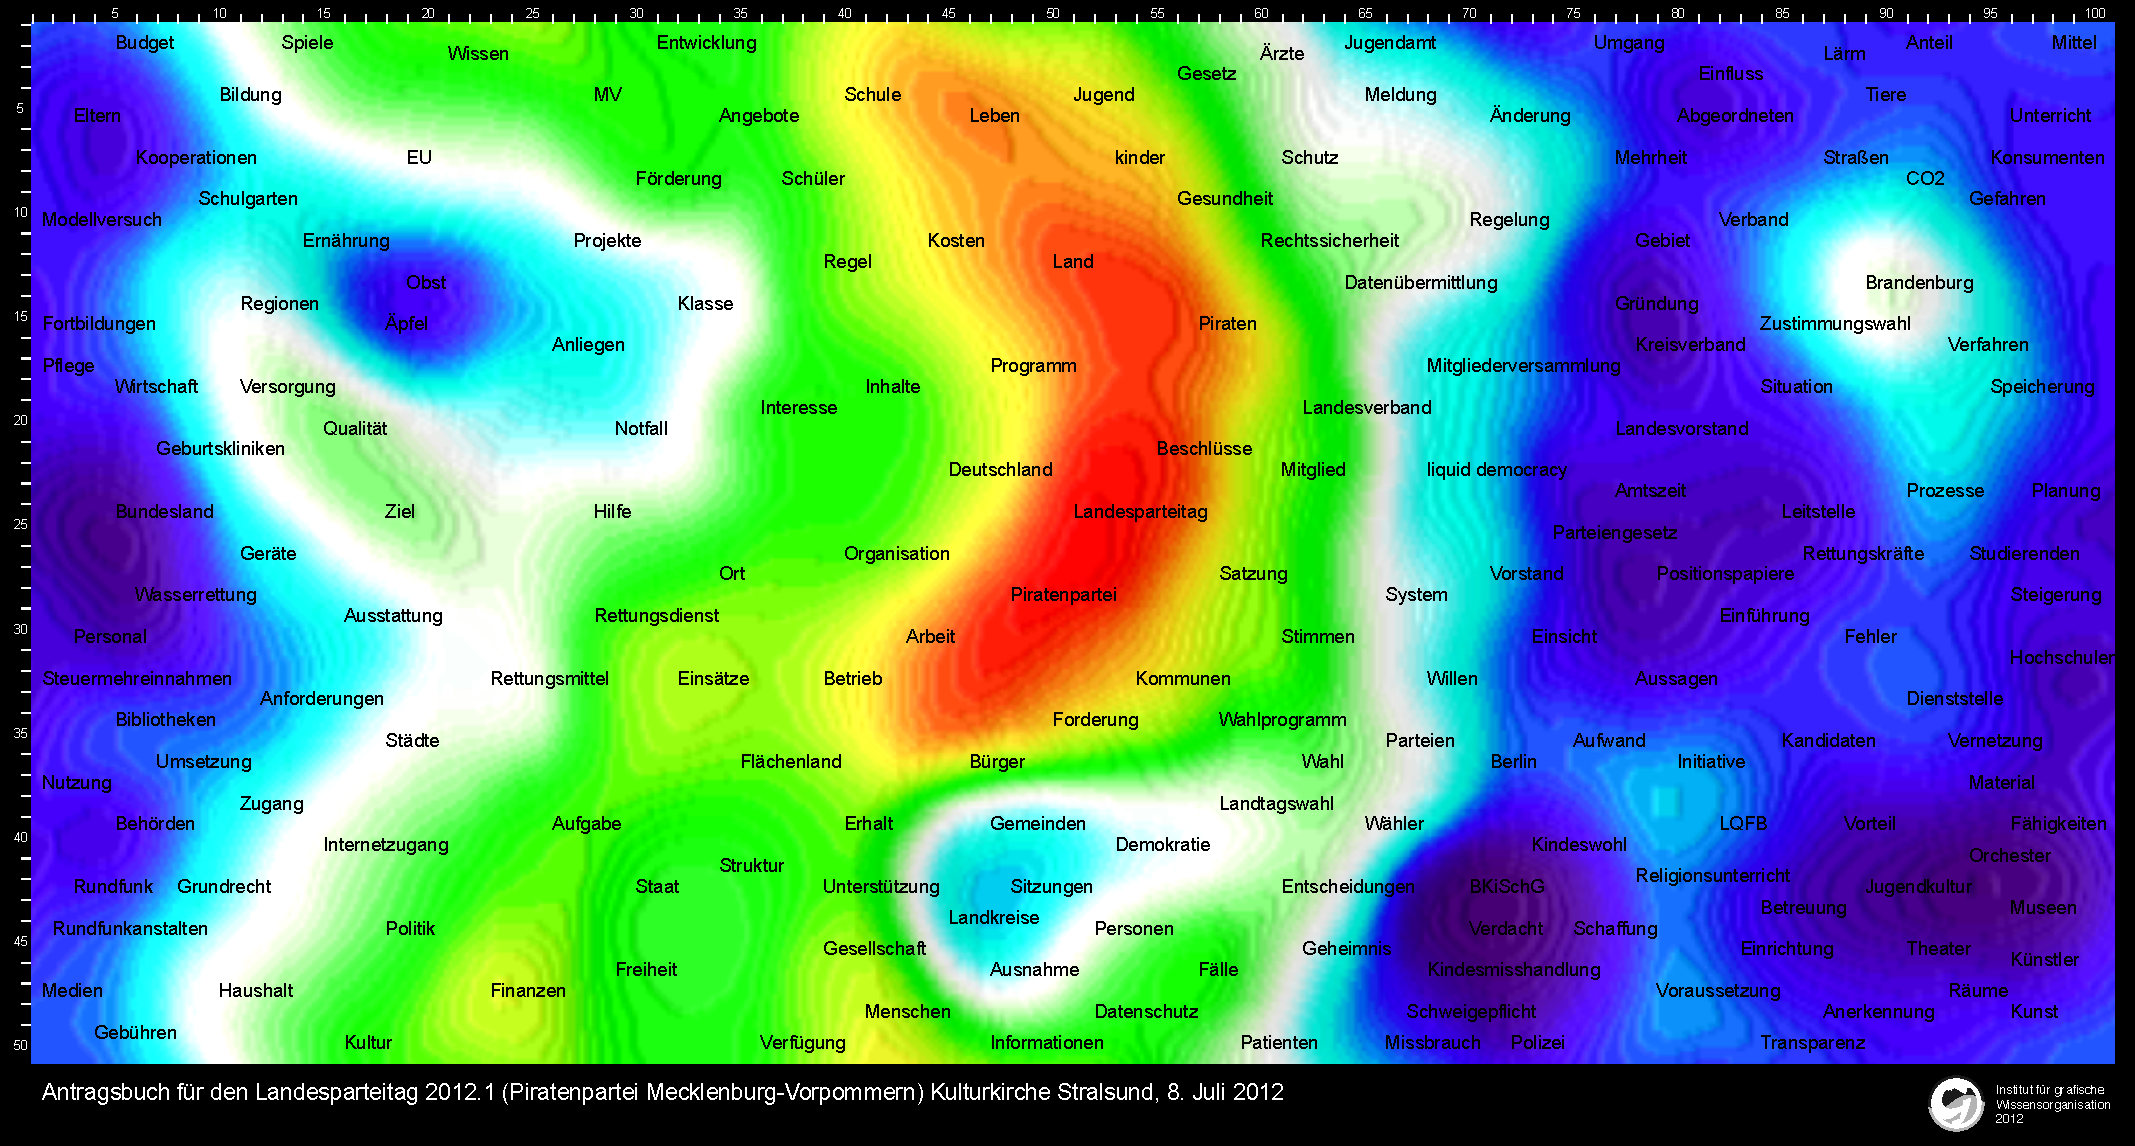
\includegraphics[width=\textwidth]{icons/som}\\Schlüsselworte der Anträge, gewichtet nach Häufigkeit

\end{abstract}

\tableofcontents
\printindex*

\newcommand{\LPTprogrammtyp}{}

%%%%%%%%%%%%%%%%%%%%%%%%%%%%%%%%%%%%%%%%%%%%%%%%%%%%%%%%%%%%%%
%%%%%%%%%%%%%%%%%%%%%%%%%%%%%%%%%%%%%%%%%%%%%%%%%%%%%%%%%%%%%%

\renewcommand{\LPTprogrammtyp}{Satzungsanträge}
\part{\LPTprogrammtyp{}}


\LPTantrag{452}
\LPTantrag{561}
\LPTantrag{562}
\LPTantrag{563}
\LPTantrag{564}
\LPTantrag{565}
\LPTantrag{566}
\LPTantrag{582}
\LPTantrag{583}
\LPTantrag{584}
\LPTantrag{586}
\LPTantrag{589}


%%%%%%%%%%%%%%%%%%%%%%%%%%%%%%%%%%%%%%%%%%%%%%%%%%%%%%%%%%%%%%

\renewcommand{\LPTprogrammtyp}{Programmanträge - Wahlprogramm}
\part{\LPTprogrammtyp{}}

\LPTantrag{587}
\LPTantrag{588}
\LPTantrag{590}
\LPTantrag{591}
\LPTantrag{592}
\LPTantrag{593}
\LPTantrag{594}
\LPTantrag{595}


%%%%%%%%%%%%%%%%%%%%%%%%%%%%%%%%%%%%%%%%%%%%%%%%%%%%%%%%%%%%%%

\renewcommand{\LPTprogrammtyp}{Programmanträge - Positionspapiere}
\part{\LPTprogrammtyp{}}



%%%%%%%%%%%%%%%%%%%%%%%%%%%%%%%%%%%%%%%%%%%%%%%%%%%%%%%%%%%%%%

\renewcommand{\LPTprogrammtyp}{Sonstige Anträge}
\part{\LPTprogrammtyp{}}

\LPTantrag{598}
\LPTantrag{610}
\LPTantrag{613}
\LPTantrag{614}
\LPTantrag{616}
\LPTantrag{617}
\LPTantrag{618}
\LPTantrag{620}
\LPTantrag{625}

%%%%%%%%%%%%%%%%%%%%%%%%%%%%%%%%%%%%%%%%%%%%%%%%%%%%%%%%%%%%%%

\setcounter{secnumdepth}{0}

\part{Anhänge}

\appendix

\chapter{Satzung des Landesverbandes Mecklenburg-Vorpommern}
\subsubsection{§ 1 - Name, Sitz und Tätigkeitsgebiet}

(1) \textsuperscript{1}Der Landesverband Mecklenburg-Vorpommern der
Piratenpartei Deutschland ist ein untergeordneter Gebietsverband auf
Landesebene gemäß der Satzung der Piratenpartei Deutschland
(Bundessatzung\textsuperscript{\href{\#cite\_note-0}{{[}1{]}}}).
\textsuperscript{2}Der Sitz des Landesverbandes und Ort der
Landesgeschäftsstelle ist Rostock.

(2) \textsuperscript{1}Der Landesverband Mecklenburg-Vorpommern der
Piratenpartei Deutschland führt einen Namen und eine Kurzbezeichnung.
\textsuperscript{2}Der Name lautet: \textbf{Piratenpartei Deutschland,
Landesverband Mecklenburg-Vorpommern}. \textsuperscript{3}Die offizielle
Abkürzung des Landesverbandes Mecklenburg-Vorpommern der Piratenpartei
Deutschland lautet: PIRATEN. \textsuperscript{4}Die Verwendung des
verkürzten Namens ``Piratenpartei MV'' ist zulässig.

(3) \textsuperscript{1}Untergeordnete Gliederungen des Landesverbandes
Mecklenburg-Vorpommern der Piratenpartei Deutschland führen den Namen
Piratenpartei Deutschland verbunden mit ihrer Organisationsstellung und
dem Namen der Gliederung. \textsuperscript{2}Den untergeordneten
Gliederungen wird die Verkürzung auf ``Piratenpartei'' in Verbindung mit
dem Gliederungsnamen erlaubt.

(4) \textsuperscript{1}Das Tätigkeitsgebiet des Landesverbandes
Mecklenburg-Vorpommern der Piratenpartei Deutschland ist das Bundesland
Mecklenburg-Vorpommern.

(5) \textsuperscript{1}Die im Landesverband Mecklenburg-Vorpommern der
Piratenpartei Deutschland organisierten Mitglieder werden
geschlechtsneutral als Piraten bezeichnet.

\subsubsection{§ 2 - Mitgliedschaft}

(1) \textsuperscript{1}Mitglied des Landesverbandes ist jedes Mitglied
der Piratenpartei Deutschland mit angezeigtem Wohnsitz in
Mecklenburg-Vorpommern.

(2) \textsuperscript{1}Der Landesverband führt ein Piratenverzeichnis.

\subsubsection{§ 3 - Erwerb der Mitgliedschaft}

(1) \textsuperscript{1}Der Erwerb der Mitgliedschaft der Piratenpartei
Deutschland wird durch die
Bundessatzung\textsuperscript{\href{\#cite\_note-1}{{[}2{]}}} geregelt.

(2) \textsuperscript{1}Jegliche Änderung am Bestand der Mitgliedsdaten
muss allen übergeordneten Gliederungen mitgeteilt werden.

\subsubsection{§ 4 - Rechte und Pflichten der Piraten}

\textsuperscript{1}Um eine Gleichbehandlung aller Piraten im
Landesverband zu gewährleisten, werden die Rechte und Pflichten der
Piraten des Landesverbandes allein durch die
Bundessatzung\textsuperscript{\href{\#cite\_note-2}{{[}3{]}}} geregelt.
\textsuperscript{2}Eine hiervon abweichende Regelung durch
untergeordnete Gliederungen ist unzulässig.

\subsubsection{§ 5 - Beendigung der Mitgliedschaft}

(1) \textsuperscript{1}Die Beendigung der Mitgliedschaft ist dem
Landesvorstand anzuzeigen.

(2) \textsuperscript{1}Die Beendigung der Mitgliedschaft in der
Piratenpartei Deutschland wird durch die
Bundessatzung\textsuperscript{\href{\#cite\_note-3}{{[}4{]}}} geregelt.

(3) \textsuperscript{1}Die Beendigung der Mitgliedschaft im
Landesverband erfolgt durch Wechsel des Wohnsitzes in ein anderes
Bundesland oder durch Beendigung der Mitgliedschaft in der Piratenpartei
Deutschland.

\subsubsection{§ 6 - Ordnungsmaßnahmen}

\textsuperscript{1}Die Regelungen zu den Ordnungsmaßnahmen, die in der
Bundessatzung\textsuperscript{\href{\#cite\_note-4}{{[}5{]}}} getroffen
werden, gelten entsprechend auch auf Landesebene.

\subsubsection{§ 7 - Gliederung}

\textsuperscript{1}Die Gliederung des Landesverbands regelt die
Bundessatzung\textsuperscript{\href{\#cite\_note-5}{{[}6{]}}}.
\textsuperscript{2}Zusammenschlüsse von Untergliederungen gleicher Ebene
sind zulässig.

\subsubsection{§ 8 - Bundespartei und Landesverbände}

\textsuperscript{1}Der Landesverband verpflichtet sich, den Regelungen
des Bundessatzung\textsuperscript{\href{\#cite\_note-6}{{[}7{]}}}
bezüglich des Verhältnisses von Bundespartei und Landesverbänden Folge
zu leisten und seine untergeordnete Gliederungen zu ebensolchem
Verhalten anzuhalten.

\subsubsection{§ 9 - Organe des Landesverbands}

\textsuperscript{1}Organe sind der Landesparteitag, das
Landesschiedsgericht und der Vorstand.

\subsubsection{§ 9a - Der Vorstand}

(1) \textsuperscript{1}Der Vorstand besteht aus dem Vorsitzenden, dem
stellvertretenden Vorsitzenden, dem Schatzmeister, dem politischen
Geschäftsführer und dem Generalsekretär.

(2) \textsuperscript{1}Der Vorstand vertritt den Landesverband nach
innen und außen. \textsuperscript{2}Er führt die Geschäfte auf Grundlage
der Beschlüsse der Parteiorgane.

(3) \textsuperscript{1}Die Mitglieder des Vorstands werden von einem
Landesparteitag mindestens jährlich in geheimer Wahl gewählt.
\textsuperscript{2}Der Vorstand bleibt bis zur Wahl eines neuen
Vorstands im Amt.

(4) \textsuperscript{1}Der Vorstand tritt in seiner Amtsperiode
mindestens zweimal zusammen. \textsuperscript{2}Er wird vom Vorsitzenden
oder bei dessen Verhinderung vom stellvertretendem Vorsitzenden mit
einer Frist von zwei Wochen unter Angabe der Tagesordnung und des
Tagungsortes einberufen. \textsuperscript{3}Bei außerordentlichen
Anlässen kann die Einberufung auch kurzfristiger erfolgen.

(5) \textsuperscript{1}Auf Antrag eines Zehntels der Piraten kann der
Vorstand zum Zusammentritt aufgefordert und mit aktuellen
Fragestellungen befasst werden. \textsuperscript{2}Die aktuelle
Mitgliederzahl ist regelmäßig zu veröffentlichen.

(6) \textsuperscript{1}Der Vorstand beschließt über alle
organisatorischen und politischen Fragen im Sinne der Beschlüsse des
Landesparteitages.

(7) \textsuperscript{1}Der Vorstand gibt sich eine Geschäftsordnung und
veröffentlicht diese angemessen. \textsuperscript{2}Sie umfasst u.a.
Regelungen zu:

\begin{enumerate}
\item
  Verwaltung der Mitgliedsdaten und deren Zugriff und Sicherung
\item
  Aufgaben und Kompetenzen der Vorstandsmitglieder
\item
  Dokumentation der Sitzungen
\item
  virtuellen oder fernmündlichen Vorstandssitzungen
\item
  Form und Umfang des Tätigkeitsberichts
\item
  Beurkundung von Beschlüssen des Vorstandes
\end{enumerate}
(8) \textsuperscript{1}Die Führung der Landesgeschäftsstelle wird durch
den Vorstand beauftragt und beaufsichtigt.

(9) \textsuperscript{1}Der Vorstand liefert zum Landesparteitag einen
schriftlichen Tätigkeitsbericht ab. \textsuperscript{2}Dieser umfasst
alle Tätigkeitsgebiete der Vorstandsmitglieder, wobei diese in
Eigenverantwortung des Einzelnen erstellt werden.
\textsuperscript{3}Wird der Vorstand insgesamt oder ein
Vorstandsmitglied nicht entlastet, so kann der Landesparteitag oder der
neue Vorstand gegen ihn Ansprüche gelten machen.
\textsuperscript{4}Tritt ein Vorstandsmitglied zurück, hat dieser
unverzüglich einen Tätigkeitsbericht zu erstellen und dem Vorstand
zuzuleiten.

(10) \textsuperscript{1}Tritt ein Vorstandsmitglied zurück bzw. kann
dieses seinen Aufgaben nicht mehr nachkommen, so geht seine Kompetenz
wenn möglich auf ein anderes Vorstandsmitglied über.
\textsuperscript{2}Der Vorstand gilt als nicht handlungsfähig, wenn mehr
als zwei Vorstandsmitglieder zurückgetreten sind oder ihren Aufgaben
nicht mehr nachkommen können oder wenn der Vorstand sich selbst für
handlungsunfähig erklärt. \textsuperscript{3}In einem solchen Fall wird
von dem dienstältesten Vorstand der direkt untergeordneten
Gliederungsebene zur Geschäftsführung eine kommissarische Vertretung
bestimmt. \textsuperscript{4}Die kommissarische Vertretung endet mit der
Neuwahl des gesamten Vorstandes auf einem unverzüglich einberufenem
außerordentlichen Parteitag.

(11) \textsuperscript{1}Tritt der gesamte Vorstand geschlossen zurück
oder kann seinen Aufgaben nicht mehr nachkommen, so führt der
dienstälteste Vorstand der direkt untergeordneten Gliederungsebene
kommissarisch die Geschäfte bis ein von ihm unverzüglich einberufener
außerordentlicher Parteitag einen neuen Vorstand gewählt hat.

\subsubsection{§ 9b - Der Landesparteitag}

(1) \textsuperscript{1}Der Landesparteitag ist die Mitgliederversammlung
auf Landesebene.

(2) \textsuperscript{1}Der Landesparteitag tagt mindestens einmal
jährlich. \textsuperscript{2}Die Einberufung erfolgt aufgrund
Vorstandsbeschluss. \textsuperscript{3}Der Vorstand lädt jedes Mitglied
persönlich mindestens vier Wochen vor dem Landesparteitag in Textform
(vorranging per E-Mail, nachrangig per Brief) ein.
\textsuperscript{4}Die Einladung hat Angaben zum Tagungsort,
Tagungsbeginn, vorläufiger Tagesordnung und der Angabe, wo weitere,
aktuelle Veröffentlichungen gemacht werden, zu enthalten.
\textsuperscript{5}Spätestens eine Woche vor dem Parteitag sind die
Tagesordnung in aktueller Fassung, die geplante Tagungsdauer und alle
bis dahin dem Vorstand eingereichten Anträge im Wortlaut zu
veröffentlichen.

(3) \textsuperscript{1}Ein außerordentlicher Landesparteitag wird
unverzüglich einberufen, wenn mindestens eins der folgenden Ereignisse
eintritt:

\begin{enumerate}
\item
  Der Vorstand ist handlungsunfähig.
\item
  Ein Zehntel der stimmberechtigten Piraten des Landesverbandes
  Mecklenburg-Vorpommern beantragt es.
\item
  Der Landesvorstand beschließt es mit einer Zweidrittelmehrheit.
\end{enumerate}
\textsuperscript{2}Es ist ein Grund für die Einberufung zu benennen.
\textsuperscript{3}Der außerordentliche Parteitag darf sich nur mit dem
benannten Grund der Einberufung befassen. \textsuperscript{4}In
dringenden Fällen kann mit einer verkürzten Frist von mindestens zwei
Wochen eingeladen werden.

(4) \textsuperscript{1}Der Landesparteitag nimmt den Tätigkeitsbericht
des Vorstandes entgegen und entscheidet daraufhin über seine Entlastung.

(5) \textsuperscript{1}Über den Landesparteitag, dessen Beschlüsse und
Wahlen wird ein Ergebnisprotokoll gefertigt, das von der
Protokollführung, der Versammlungsleitung und der Wahlleitung
unterschrieben und anschließend veröffentlicht wird.

(6) \textsuperscript{1}Der Landesparteitag wählt mindestens zwei
Rechnungsprüfer, die den finanziellen Teil des Tätigkeitsberichtes des
Vorstandes vor der Beschlussfassung über ihn prüfen.
\textsuperscript{2}Das Ergebnis der Prüfung wird dem Landesparteitag
verkündet und zu Protokoll genommen. \textsuperscript{3}Danach sind die
Rechnungsprüfer aus ihrer Funktion entlassen.

(7) \textsuperscript{1}Der Landesparteitag wählt mindestens zwei
Kassenprüfer. \textsuperscript{2}Diesen obliegen die Vorprüfung des
finanziellen Tätigkeitsberichtes für den folgenden Landesparteitag und
die Vorprüfung, ob die Finanzordnung und das PartG eingehalten wird.
\textsuperscript{3}Sie haben das Recht, Einsicht in alle
finanzrelevanten Unterlagen zu verlangen, und auf Wunsch Kopien
persönlich ausgehändigt zu bekommen. \textsuperscript{4}Sie sind
angehalten, etwa zwei Wochen vor dem Landesparteitag die letzte
Vorprüfung der Finanzen durchzuführen. \textsuperscript{5}Ihre Amtszeit
endet durch Austritt, Rücktritt, Entlassung durch den Landesparteitag
oder mit Wahl ihrer Nachfolger.

\subsubsection{§ 10 - Bewerberaufstellung für die Wahlen zu
Volksvertretungen}

(1) \textsuperscript{1}Die Bewerberaufstellung für die Wahlen zu
Volksvertretungen erfolgt nach den Regularien der einschlägigen Gesetze
sowie den Vorgaben der
Bundessatzung\textsuperscript{\href{\#cite\_note-7}{{[}8{]}}}.

(2) \textsuperscript{1}Die Aufstellung kann sowohl als
Mitgliederversammlung des zuständigen Stimm- bzw. Wahlkreises als auch
im Rahmen einer anderen Mitgliederversammlung stattfinden, sofern
gewährleistet wird, dass alle Stimmberechtigten in angemessener Zeit und
Form eingeladen wurden und nur die Stimmberechtigten an der Wahl
teilnehmen. \textsuperscript{2}Die Einladung muss dabei explizit auf die
Bewerberaufstellung hinweisen.

\subsubsection{§ 11 - Satzungs- und Programmänderung}

(1) \textsuperscript{1}Änderungen der Landessatzung und des Programms
können nur von einem Landesparteitag mit einer Zweidrittelmehrheit
beschlossen werden. \textsuperscript{2}Besteht das dringende Erfordernis
einer Satzungsänderung zwischen zwei Landesparteitagen, so kann die
Satzung auch geändert werden, wenn mindestens zwei Dritteln der Piraten
dem Änderungsantrag schriftlich zustimmen.

(2) \textsuperscript{1}Über einen Antrag auf Satzungs- oder
Programmänderung auf einem Landesparteitag kann nur abgestimmt werden,
wenn er mindestens zwei Wochen vor Beginn des Landesparteitages beim
Vorstand eingegangen ist.

(3) \textsuperscript{1}Der Landesverband übernimmt das Grundsatzprogramm
der Piratenpartei Deutschland. \textsuperscript{2}Vom Landesparteitag
kann ein eigenes Wahlprogramm für Kommunal- und Landtagswahlen
verabschiedet werden. \textsuperscript{3}Dieses muss auf den Werten des
Grundsatzprogrammes basieren.

\subsubsection{§ 12 - Auflösung und Verschmelzung}

\textsuperscript{1}Die Auflösung oder Verschmelzung regelt die
Bundessatzung\textsuperscript{\href{\#cite\_note-8}{{[}9{]}}}.

\subsubsection{§ 13 - Parteiämter}

\textsuperscript{1}Die Regelung der
Bundessatzung\textsuperscript{\href{\#cite\_note-9}{{[}10{]}}} zu den
Parteiämtern findet Anwendung.

\bigskip

\subsection{Abschnitt B: Finanzordnung}

\subsubsection{§ 16 Finanzordnung}

\textsuperscript{1}Die Finanzordnung der
Bundessatzung\textsuperscript{\href{\#cite\_note-10}{{[}11{]}}} findet
entsprechende Anwendung.

\subsection{Abschnitt C: Schiedsgerichtsordnung}

\subsubsection{§ 15 Landesschiedsgericht}

\textsuperscript{1}Für das Landesschiedsgericht gilt die
Bundesschiedsgerichtsordnung\textsuperscript{\href{\#cite\_note-11}{{[}12{]}}}.

\subsection{Abschnitt D: Organisatorisches}

\subsubsection{§ 16 Wahlordnung}

\textsuperscript{1}Der Landesparteitag regelt das Verfahren von Wahlen
und Abstimmungen in einer
Wahlordnung\textsuperscript{\href{\#cite\_note-12}{{[}13{]}}}.

\subsubsection{§ 17 Schlussbestimmungen}

\textsuperscript{1}Diese Satzung tritt mit Verabschiedung durch den
Landesparteitag in Kraft.

\subsection{Referenzen}

\begin{enumerate}
\item
  \href{\#cite\_ref-0}{↑} \href{/Bundessatzung}{Bundessatzung}
\item
  \href{\#cite\_ref-1}{↑}
  \href{/Bundessatzung\#.C2.A7\_3\_-\_Erwerb\_der\_Mitgliedschaft}{§ 3
  Bundessatzung (``Erwerb der Mitgliedschaft'')}
\item
  \href{\#cite\_ref-2}{↑}
  \href{/Bundessatzung\#.C2.A7\_4\_-\_Rechte\_und\_Pflichten\_der\_Piraten}{§
  4 Bundessatzung (``Rechte und Pflichten der Piraten'')}
\item
  \href{\#cite\_ref-3}{↑}
  \href{/Bundessatzung\#.C2.A7\_5\_-\_Beendigung\_der\_Mitgliedschaft}{§
  5 Bundessatzung (``Beendigung der Mitgliedschaft'')}
\item
  \href{\#cite\_ref-4}{↑}
  \href{/Bundessatzung\#.C2.A7\_6\_-\_Ordnungsma.C3.9Fnahmen}{§ 6
  Bundessatzung (``Ordnungsmaßnahmen'')}
\item
  \href{\#cite\_ref-5}{↑}
  \href{/Bundessatzung\#.C2.A7\_7\_-\_Gliederung}{§ 7 Bundessatzung
  (``Gliederung'')}
\item
  \href{\#cite\_ref-6}{↑}
  \href{/Bundessatzung\#.C2.A7\_8\_-\_Bundespartei\_und\_Landesverb.C3.A4nde}{§
  8 Bundessatzung (``Bundespartei und Landesverbände'')}
\item
  \href{\#cite\_ref-7}{↑}
  \href{/Bundessatzung\#.C2.A7\_10\_-\_Bewerberaufstellung\_f.C3.BCr\_die\_Wahlen\_zu\_Volksvertretungen}{§
  10 Bundessatzung (``Bewerberaufstellung für die Wahlen zu
  Volksvertretungen'')}
\item
  \href{\#cite\_ref-8}{↑}
  \href{/Bundessatzung\#.C2.A7\_13\_-\_Aufl.C3.B6sung\_und\_Verschmelzung}{§
  13 Bundessatzung (``Auflösung und Verschmelzung'')}
\item
  \href{\#cite\_ref-9}{↑}
  \href{/Bundessatzung\#.C2.A7\_15\_-\_Partei.C3.A4mter}{§ 15
  Bundessatzung (``Parteiämter'')}
\item
  \href{\#cite\_ref-10}{↑}
  \href{/Bundessatzung\#Abschnitt\_B:\_Finanzordnung}{Abschnitt B
  Bundessatzung (``Finanzordnung'')}
\item
  \href{\#cite\_ref-11}{↑}
  \href{/Bundessatzung\#Abschnitt\_C:\_Schiedsgerichtsordnung}{Abschnitt
  C Bundessatzung (``Schiedsgerichtsordnung'')}
\item
  \href{\#cite\_ref-12}{↑} \href{/MV:Wahlordnung}{Wahl- und
  Abstimmungsordnung der Piraten in Mecklenburg-Vorpommern}
\end{enumerate}


%\chapter{Wahlordnung des Landesverbandes Mecklenburg-Vorpommern}
%\subsection{Allgemeiner Teil.}

\subsubsection{§ 1}

(1) Diese Wahl- und Abstimmungsordnung gilt für alle Versammlungen der
Piraten in Mecklenburg-Vorpommern. Sie gilt, vorbehaltlich besonderer
Bestimmungen der Wahlgesetze, auch für Versammlungen zur Aufstellung von
Kandidaten.

(2) Im Sinne dieser Ordnung ist:

\begin{enumerate}
\item
  Wahl: eine Entscheidung über Personalfragen;
\item
  Abstimmung: eine Entscheidung über Sachfragen;
\item
  Pirat: wer nach § 1 Absatz 5 der Satzung des Landesverbandes Pirat
  ist;
\item
  einfache Mehrheit: die Mehrheit der anwesenden Stimmen;
\item
  geheim: eine Wahl oder Abstimmung, bei der die Stimmen der
  stimmberechtigten Piraten diesen nicht zugeordnet werden können;
\item
  öffentlich: eine Wahl oder Abstimmung, wenn sie für jedermann
  zugänglich ist.
\end{enumerate}
\subsubsection{§ 2}

(1) Wahlen und Abstimmungen sind frei, gleich und allgemein und finden
öffentlich statt.

(2) Wahl- und abstimmungsberechtigt ist, wer dem beschließenden Gremium
beim Zusammentritt als stimmberechtigtes Mitglied angehören kann.

(3) Piraten können sich bei einer nicht geheimen Wahl oder Abstimmung
vertreten lassen. Sie benötigen dazu die Vollmacht des betreffenden
stimmberechtigten Piraten, die zu Beginn der Sitzung dem Wahl- oder
Abstimmungsleiter vorgelegt werden muss.

\subsubsection{§ 3}

(1) Werden Stimmzettel verwendet, müssen sie einheitlich sein. Bei
geheimen Wahlen und Abstimmungen müssen Stimmzettel verwendet werden.

(2) Ungültig sind Stimmzettel, die den Willen des wählenden Piraten
nicht zweifelsfrei erkennen lassen.

\subsubsection{§ 4}

(1) Wählen oder abstimmen können auch aus wichtigem Grunde abwesende,
stimmberechtigte Piraten, wenn die Wahl oder Abstimmung in der
Tagesordnung festgelegt ist, sie rechtzeitig bekannt gemacht wurde und
der Vorstand dies zugelassen hat.

(2) Zulässig sind Möglichkeiten der Wahl oder Abstimmung, wenn dies über
Wege geschieht, die eine geheime Wahl oder Abstimmung ermöglichen und
zulassen, und der wählende oder abstimmende Pirat dabei seine Identität
nachweisen kann, ohne dass die Geheimheit der Wahl betroffen ist.

\subsubsection{§ 5}

(1) Bei der Bestimmung des Ergebnisses werden nicht abgegebene Stimmen
als nicht anwesend gewertet, sofern nichts anderes bestimmt ist.
Enthaltungen gelten als nicht abgegebene Stimmen.

(2) Die Ergebnisse einer Wahl oder Abstimmung müssen so veröffentlicht
werden, dass alle für die Wahl oder Abstimmung stimmberechtigten Piraten
sie einsehen können.

\subsubsection{§ 6}

(1) Jedem zu einer Wahl oder Abstimmung stimmberechtigten Pirat steht
das Recht zur Anfechtung der Wahl oder Abstimmung zu, wenn die
Verletzung von Bestimmungen der Satzung, des Parteiengesetzes, der
Wahlgesetze, des Verfassungsrechts oder eines anderen gültigen Gesetzes
oder Beschlusses als möglich erscheint. Sie ist bis zum 14. Tage nach
der Wahl oder Abstimmung zulässig und muss beim zuständigen Vorstand
eingereicht werden.

(2) Hält der Vorstand die Anfechtung für begründet, erklärt er die Wahl
oder Abstimmung für ungültig.

(3) Gegen die die Anfechtung versagende Entscheidung des Vorstandes ist
die Beschwerde beim Schiedsgericht zulässig.

\subsection{Besonderer Teil.}

\subsubsection{Erster Abschnitt. Wahlen.}

\paragraph{§ 7}

(1) Wahlen finden geheim statt, soweit diese Wahl- und
Abstimmungsordnung nicht etwas anderes bestimmt.

(2) Wahlen können nur stattfinden, wenn sie in der Tagesordnung
angekündigt worden sind, soweit diese Wahl- und Abstimmungsordnung nicht
etwas anderes bestimmt. Die Tagesordnung muss den stimmberechtigten
Piraten spätestens sieben Tage vor der Wahl in Textform zugehen. Bei
Nominierungen zu öffentlichen Ämtern gelten die entsprechenden
gesetzlichen Fristen.

\paragraph{§ 8}

(1) Die Kandidaten sollen gemeinsam in einem Wahldurchgang gewählt
werden.

(2) Gibt es bei Vorstandswahlen für ein Amt nur einen Kandidaten, findet
§ 13 entsprechende Anwendung mit der Maßgabe, dass Enthaltungen als
abgegebene Stimmen gelten. Bewerben sich mehrere Kandidaten um ein Amt,
findet eine Mehrheitswahl statt, bei der Enthaltungen als abgegebene
Stimmen gelten. Gewählt ist, wer die einfache Mehrheit auf sich
vereinigt.

(3) Direktkandidaten für Wahlen zum Europäischen Parlament, zum Bundes-
oder Landtag oder zu kommunalen Vertretungen werden entsprechend Absatz
2 gewählt. Listenkandidaten werden durch eine Akzeptanzwahl aufgestellt,
die in zwei Wahlgängen erfolgt. Im ersten Wahlgang werden so viele
künftige Listenkandidaten gewählt, wie in einer vorhergehenden
Abstimmung beschlossen wurde. Dieser Wahlgang entfällt, wenn sich
weniger Kandidaten für die Liste bewerben, als nach dem Beschluss
aufgestellt werden können. Im zweiten Wahlgang wird die Reihenfolge der
Kandidaten festgelegt, indem jeder stimmberechtigte Pirat eine um eins
erhöhte der Kandidatenzahl entsprechende Stimmenzahl bekommt, die er auf
einen oder mehrere Kandidaten verteilen kann. Die Aufstellung der
Listenkandidaten erfolgt nach absteigender Stimmenzahl.

(4) Versammlungsleiter, Moderatoren, Wahlleiter, Protokollführer und
andere zur Wahl gestellte Personen werden entsprechend Absatz 2 gewählt.
Solche Wahlen finden grundsätzlich nicht geheim statt und müssen nicht
in der Tagesordnung angekündigt werden.

\paragraph{§ 9}

Gibt es bei einer Wahl durch Stimmengleichheit kein eindeutiges
Ergebnis, ist für diese Kandidaten eine Stichwahl durchzuführen. Führt
diese ebenfalls zu keinem Ergebnis, entscheidet das Los.

\paragraph{§ 10}

Für Nachwahlen gelten die gleichen Bestimmungen wie für Wahlen. Die
Wahlperioden bleiben davon unberührt.

\subsubsection{Zweiter Abschnitt. Abstimmungen.}

\paragraph{§ 11}

Soweit in diesem Abschnitt nichts anderes bestimmt ist, finden die
Vorschriften zu den Wahlen entsprechende Anwendung.

\paragraph{§ 12}

Abstimmungen finden nicht geheim statt. Auf Antrag eines Zehntels der
anwesenden, stimmberechtigten Piraten kann mit einfacher Mehrheit geheim
abgestimmt werden. Über den Antrag wird in geheimer Abstimmung
entschieden.

\paragraph{§ 13}

(1) Abstimmungsfragen müssen so gestellt werden, dass sie mit Ja oder
Nein beantwortet werden können.

(2) Die zur Abstimmung gestellte Frage ist positiv beschieden, wenn die
Ja-Stimmen die Nein-Stimmen überwiegen.

(3) Die Anzahl der abgegebenen Stimmen muss mindestens fünfzig vom
Hundert der anwesenden Stimmen betragen.


\chapter{Geschäftsordnung}
Folgende Anträge zur Geschäftsordnung sind zulässig:

\begin{description}
    \item[§ 18] Zulassung des Gastredners
    \item[§ 19] Ablehnung eines Wahlhelfers
    \item[§ 20] Geheime Wahl
    \item[§ 21] Geheime Abstimmung
    \item[§ 22] Wiederholung der Wahl/Abstimmung
    \item[§ 23] Auszählung einer Abstimmung
    \item[§ 24] Getrennte Wahlgänge
    \item[§ 25] Änderung der Reihenfolge der Wahlgänge
    \item[§ 26] GO-Alternativantrag
    \item[§ 27] Schließung der Redeliste
    \item[§ 28] Wiedereröffnung der Redeliste
    \item[§ 29] Begrenzung der Redezeit
    \item[§ 30] Einholung eines Meinungsbildes
    \item[§ 31] Unterbrechung der Sitzung
    \item[§ 32] Änderung der Tagesordnung
    \item[§ 33] Änderung der Geschäftsordnung
\end{description}

\section{Hinweis}

\minisec{§ 17 Anträge zur Geschäftsordnung}

(4) Um Missverständnisse zu vermeiden, sollen komplexere GO-Anträge als Text beim Versammlungsleiter oder dem von ihm damit beauftragten Piraten eingereicht werden.


%\chapter{Anträge zur Geschäftsordnung}
%\input{anhaenge/go-antraege.tex}

\newpage
\null
\thispagestyle{empty}
\ThisTileWallPaper{200pt}{200pt}{icons/slogans.png}

\end{document}  